\chapteropening[Applications to Group Theory]{Applications \\to Group Theory}

In the preceding chapter, we showed how a problem of topology---classifying all covering spaces of a space \(B\) ---can be reduced to a problem of algebra---classifying all subgroups of the fundamental group of \(B\). Now we consider the reverse process, that of reducing a problem of algebra to one of topology. The problem of algebra in question is that of showing that any subgroup of a free group is itself a free group. While this statement is certainly believable, it is not one whose proof is obvious. We shall proceed by applying the theory of covering spaces to certain topological spaces called linear graphs.

\booksection{83}{Covering Spaces of a Graph}

We define here the notion of linear graph (introduced earlier in the finite case), and prove the basic theorem that any covering space of a linear graph is itself a linear graph.

Recall that an arc \(A\) is a space homeomorphic to the unit interval \([ {0,1}]\). The end points of \(A\) are the points \(p,q\) corresponding to 0 and 1 under the homeomorphism; they are the unique points of \(A\) such that \(A - p\) and \(A - q\) are connected. The interior of an arc \(A\) consists of \(A\) with its end points deleted.

\begin{definition}
	A linear graph is a space \(X\) that is written as the union of a collection of subspaces \(A_{\alpha }\), each of which is an arc, such that:

	\begin{enumerate}[itemsep=0.2em, parsep=0pt, topsep=0pt, partopsep=0pt, leftmargin=*, label=(\arabic*), align=left]
	\item The intersection \(A_{\alpha } \cap {A}_{\beta }\) of two arcs is either empty or consists of a single point that is an end point of each.
	\item The topology of \(X\) is coherent with the subspaces \(A_{\alpha }\).
	\end{enumerate}

The arcs \(A_{\alpha }\) are called the edges of \(X\), and their interiors are called the open edges of \(X\). Their end points are called the vertices of \(X\) ; we denote the set of vertices of \(X\) by \(X^{0}\).
\end{definition}

If \(X\) is a linear graph, and if \(C\) is a subset of \(X\) that equals a union of edges and vertices of \(X\), then \(C\) is closed in \(X\). For the intersection of \(C\) with \(A_{\alpha }\) is closed in \(A_{\alpha }\), since it is either empty, or it equals \(A_{\alpha }\), or it equals one or both vertices of \(A_{\alpha }\). It follows that each edge of \(X\) is a closed subset of \(X\). It also follows that \(X^{0}\) is a closed discrete subspace of \(X\), since any subset of \(X^{0}\) is closed in \(X\).

In the case of a finite graph, considered earlier, we used the Hausdorff condition in our definition in place of condition (2); it followed, in that case, that the topology of \(X\) was coherent with the subspaces \(A_{\alpha }\). In the case of an infinite graph, this would no longer be true, so we must assume the coherence condition as part of the definition. We would assume the Hausdorff condition as well, but it is no longer necessary, for it follows from the coherence condition:

\begin{lemma}
\label{lem:\thetheorem}
Every linear graph \(X\) is Hausdorff; in fact, it is normal.
\end{lemma}

\begin{proof}
	Let \(B\) and \(C\) be disjoint closed subsets of \(X\). Assume, without loss of generality, that every vertex of \(X\) belongs either to \(B\) or to \(C\). For each \(\alpha\), choose disjoint subsets \(U_{\alpha }\) and \(V_{\alpha }\) of \(A_{\alpha }\) that are open in \(A_{\alpha }\), containing \(B \cap {A}_{\alpha }\) and \(C \cap {A}_{\alpha }\), respectively. Let \(U = \bigcup {U}_{\alpha }\) and \(V = \bigcup {V}_{\alpha }\). Then \(U\) and \(V\) contain \(B\) and \(C\), respectively.
We show the sets \(U\) and \(V\) are disjoint. If \(x \in U \cap V\), then \(x \in {U}_{\alpha } \cap {V}_{\beta }\) for some \(\alpha \neq \beta\). This fact implies that \(A_{\alpha }\) and \(A_{\beta }\) contain the point \(x\), which means that \(x\) is a vertex of \(X\). This is impossible, for if \(x \in B\), then \(x\) lies in no set \(V_{\beta }\), and if \(x \in C\), then \(x\) lies in no set \(U_{\alpha }\).

Now we show \(U\) and \(V\) are open in \(X\). To show \(U\) is open, we show that \(U \cap {A}_{\alpha } =\) \(U_{\alpha }\) for each \(\alpha\). By definition, \(U \cap {A}_{\alpha }\) contains \(U_{\alpha }\). If \(x\) is a point of \(U \cap {A}_{\alpha }\) not in \(U_{\alpha }\), then \(x\) belongs to \(U_{\beta }\) for some \(\beta \neq \alpha\). Then both \(A_{\beta }\) and \(A_{\alpha }\) contain \(x\), so that \(x\) must be a vertex of \(X\). This is impossible, for if \(x \in B\), then \(x \in {U}_{\alpha }\) by definition of \(U_{\alpha }\), and if \(x \in C\), then \(x\) cannot belong to \(U\).

\begin{centeredblock}
\begin{example}
\label{ex:\thesection.\theexample}
	If \(X\) is the wedge of the circles \(S_{\alpha }\), with common point \(p\), then \(X\) can be expressed as a linear graph. We need merely write each \(S_{\alpha }\) as a graph having three edges, with \(p\) as one of its vertices; then \(X\) is a union of arcs. To show that the topology of the wedge \(X\) is coherent with the resulting collection of arcs, we note that if \(D \cap {A}_{\alpha }\) is closed in \(A_{\alpha }\) for each arc \(A_{\alpha }\), then \(D \cap {S}_{\beta }\) is the union of three sets of the form \(D \cap {A}_{\alpha }\) and so is closed in \(S_{\beta }\) ; then \(D\) is closed in \(X\) by definition. See \hyperref[fig:83.1]{Figure 83.1}.
\end{example}
\end{centeredblock}

\begin{centeredblock}
\begin{example}
\label{ex:\thesection.\theexample}
	Let \(J\) be a discrete space, and let \(E = [ {0,1}] \times J\). Then the quotient space \(X\) obtained from \(E\) by collapsing the set \(\{ 0\} \times J\) to a point \(p\) is a linear graph.

The quotient map \(\pi : E \rightarrow X\) is a closed map. For if \(C\) is closed in \(E\), then \({\pi }^{-1}\pi ( C)\) equals \(C \cup ( {\{ 0\} \times J})\) if \(C\) contains a point of \(\{ 0\} \times J\), and \({\pi }^{-1}\pi ( C)\) equals \(C\) otherwise. In either case, \({\pi }^{-1}\pi ( C)\) is closed in \(E\), so that \(\pi ( C)\) is closed in \(X\). It follows that \(\pi\) maps each space \([ {0,1}] \times \alpha\) homeomorphically onto its image \(A_{\alpha }\), so that \(A_{\alpha }\) is an arc. The topology of \(X\) is coherent with the subspaces \(A_{\alpha }\) because \(\pi\) is a quotient map. See \hyperref[fig:83.2]{Figure 83.2}.
\end{example}
\end{centeredblock}

\munkresfig[0.3]{83.1}[Figure 83.1]
\munkresfig[0.2]{83.2}[Figure 83.2]
\end{proof}
\begin{definition}
	Let \(X\) be a linear graph. Let \(Y\) be a subspace of \(X\) that is a union of edges of \(X\). Then \(Y\) is closed in \(X\) and is itself a linear graph; we call it a subgraph of \(X\).
\end{definition}

To show that \(Y\) is a linear graph, we need to show that the subspace topology on \(Y\) is coherent with the set of edges of \(Y\). If the subset \(D\) of \(Y\) is closed in the subspace topology, then \(D\) is closed in \(X\), so that \(D \cap {A}_{\alpha }\) is closed in \(A_{\alpha }\) for each edge of \(X\), and in particular for each edge of \(Y\). Conversely, suppose \(D \cap {A}_{\beta }\) is closed in \(A_{\beta }\) for each edge \(A_{\beta }\) of \(Y\). We must show that \(D \cap {A}_{\alpha }\) is closed in \(A_{\alpha }\) for each edge \(A_{\alpha }\) of \(X\) that is not contained in \(Y\). But in this case, \(D \cap {A}_{\alpha }\) is either empty or a one-point set! We conclude that \(Y\) has the topology coherent with its set of edges.

\begin{lemma}
\label{lem:\thetheorem}
	Let \(X\) be a linear graph. If \(C\) is a compact subspace of \(X\), there exists a finite subgraph \(Y\) of \(X\) that contains \(C\). If \(C\) is connected, \(Y\) can be chosen to be connected.
\end{lemma}

\begin{proof}
	First, note that \(C\) contains only finitely many vertices of \(X\). For \(C \cap {X}^{0}\) is a closed discrete subspace of the compact space \(C\) ; since it has no limit point, it must be finite. Similarly, there are only finitely many values of \(\alpha\) for which \(C\) contains an interior point of the edge \(A_{\alpha }\). For if we choose a point \(x_{\alpha }\) of \(C\) interior to \(A_{\alpha }\) for each index \(\alpha\) for which it is possible to do so, we obtain a collection \(B = \{ x_{\alpha }\}\) whose intersection with each edge \(A_{\beta }\) is a one-point set or empty. It follows that every subset of \(B\) is closed in \(X\), so that \(B\) is a closed discrete subspace of \(C\) and hence finite.
Form \(Y\) by choosing, for each vertex \(x\) of \(X\) belonging to \(C\), an edge of \(X\) having \(x\) as a vertex, and adjoining to these edges all edges \(A_{\alpha }\) whose interiors contain points of \(C\). Then \(Y\) is a finite subgraph containing \(C\). Note that if \(C\) is connected, then \(Y\) is the union of a collection of arcs each of which intersects \(C\), so that \(Y\) is connected.
\end{proof}
\begin{lemma}
\label{lem:\thetheorem}
	If \(X\) is a linear graph, then \(X\) is locally path connected and semilocally simply connected.
\end{lemma}

\begin{proof}
	Step 1. We show \(X\) is locally path connected. If \(x \in X\) and \(x\) lies interior to some edge of \(X\), then within every neighborhood of \(x\) is a neighborhood of \(x\) homeomorphic to an open interval of \(\mathbb{R}\), which is path connected. On the other hand, if \(x\) is a vertex of \(X\) and \(U\) is a neighborhood of \(x\), then we can choose, for each edge \(A_{\alpha }\) having \(x\) as an end point, a neighborhood \(V_{\alpha }\) of \(x\) in \(A_{\alpha }\) lying in \(U\) that is homeomorphic to the half-open interval \([ {0,1}]\). Then \(\bigcup {V}_{\alpha }\) is a neighborhood of \(x\) in \(X\) lying in \(U\), and it is a union of path-connected spaces having the point \(x\) in common.
Step 2. We show \(X\) is semilocally simply connected. Indeed, we show that if \(x \in X\), then \(x\) has a neighborhood \(U\) such that \({\pi }_{1}( {U,x})\) is trivial.

If \(x\) lies interior to some edge of \(X\), then the interior of this edge is such a neighborhood. So suppose \(x\) is a vertex of \(X\). Let \(\overline{\operatorname{St}}x\) denote the union of those edges of \(X\) that have \(x\) as an end point, and let \(\operatorname{St}x\) denote the subspace of \(\overline{\operatorname{St}}x\) obtained by deleting all vertices other than \(x\). (St \(x\) is called the star of \(x\) in \(X\).) The set \(\operatorname{St}x\) is open in \(X\), since its complement is a union of arcs and vertices. We show that \({\pi }_{1}( {\operatorname{St}x, x})\) is trivial.

Let \(f\) be a loop in \(\operatorname{St}x\) based at \(x\). Then the image set \(f( I)\) is compact, so it lies in some finite union of arcs of \(\overline{\operatorname{St}}x\). Any such union is homeomorphic to the union of a finite set of line segments in the plane having an end point in common. And for any loop in such a space, the straight-line homotopy will shrink it to the constant loop at \(x\).

Now if \(x\) is a vertex of \(X\), it is in fact true that the one-point space \(\{ x\}\) is a deformation retract of \(\overline{\operatorname{St}}x\). But there is a surprising amount of effort required to show that the obvious deformation is continuous. One needs the fact that a map

\[
F : ( {\overline{\operatorname{St}}x}) \times I \rightarrow \overline{\operatorname{St}}x
\]

is continuous if its restriction to each subspace \(A_{\alpha } \times I\) is continuous. This result follows from the pasting lemma in the case where \(\overline{\operatorname{St}}x\) is a union of only finitely many arcs, but the general result requires one to show that the topology of \(( {\overline{\operatorname{St}}x}) \times I\) is coherent with the subspaces \(A_{\alpha } \times I\). This in turn follows from a basic theorem about products of quotient maps. (See Exercise 11 of \S\ 29.) These considerations do not arise if one wishes merely to shrink a loop to a point (rather than shrinking the entire space St \(x\) ), since any loop lies in the union of a finite number of edges, where there is no problem.
\end{proof}

Now we discuss covering spaces of linear graphs. Note that the convention that every covering space is assumed to be path connected and locally path connected, which we assumed in the last chapter, no longer applies.
\begin{theorem}
\label{thm:\thetheorem}
	Let \(p : E \rightarrow X\) be a covering map, where \(X\) is a linear graph. If \(A_{\alpha }\) is an edge of \(X\) and \(B\) is a path component of \(p^{-1}( A_{\alpha })\), then \(p\) maps \(B\) homeomorphically onto \(A_{\alpha }\). Furthermore, the space \(E\) is a linear graph, with the path components of the spaces \(p^{-1}( A_{\alpha })\) as its edges.
\end{theorem}

\begin{proof}
	Step 1. We show that \(p\) maps \(B\) homeomorphically onto \(A_{\alpha }\). Because the arc \(A_{\alpha }\) is path connected and locally path connected, \hyperref[thm:53.2]{Theorem 53.2} and \hyperref[lem:80.1]{Lemma 80.1} tell us that the map \(p_{0} : B \rightarrow {A}_{\alpha }\) obtained by restricting \(p\) is a covering map. Because \(B\) is path connected, the lifting correspondence \(\phi : {\pi }_{1}( {A_{\alpha },a}) \rightarrow {p}_0^{-1}( a)\) is surjective; because \(A_{\alpha }\) is simply connected, \(p_0^{-1}( a)\) consists of a single point. (See \hyperref[thm:54.4]{Theorem 54.4}.) Hence \(p_{0}\) is a homeomorphism.
Step 2. Because \(X\) is the union of the arcs \(A_{\alpha }\), the space \(E\) is the union of the arcs \(B\) that are the path components of the spaces \(p^{-1}( A_{\alpha })\). Let \(B\) and \(B^{\prime }\) be path components of \(p^{-1}( A_{\alpha })\) and \(p^{-1}( A_{\beta })\), respectively, with \(B \neq {B}^{\prime }\). We show \(B\) and \(B^{\prime }\) intersect in at most a common end point. If \(A_{\alpha }\) and \(A_{\beta }\) are equal, then \(B\) and \(B^{\prime }\) are disjoint, and if \(A_{\alpha }\) and \(A_{\beta }\) are disjoint, so are \(B\) and \(B^{\prime }\). Therefore, if \(B\) and \(B^{\prime }\) intersect, \(A_{\alpha }\) and \(A_{\beta }\) must intersect in an end point \(x\) of each; then \(B \cap {B}^{\prime }\) consists of a single point, which must be an end point of each.

Step 3. We show that \(E\) has the topology coherent with the arcs \(B\). This is the hardest part of the proof. Let \(W\) be a subset of \(E\) such that \(W \cap B\) is open in \(B\), for each arc \(B\) of \(E\). We show that \(W\) is open in \(E\).

First, we show that \(p( W)\) is open in \(X\). If \(A_{\alpha }\) is an edge of \(X\), then \(p( W) \cap {A}_{\alpha }\) is the union of the sets \(p( {W \cap B})\), as \(B\) ranges over all path components of \(p^{-1}( A_{\alpha })\). Each of these sets \(p( {W \cap B})\) is open in \(A_{\alpha }\), because \(p\) maps \(B\) homeomorphically onto \(A_{\alpha }\) ; hence their union \(p( W) \cap {A}_{\alpha }\) is open in \(A_{\alpha }\). Because \(X\) has the topology coherent with the subspaces \(A_{\alpha }\), the set \(p( W)\) is open in \(X\).

Second, we prove our result in the special case where the set \(W\) is contained in one of the slices \(V\) of \(p^{-1}( U)\), where \(U\) is an open set of \(X\) that is evenly covered by \(p\). By the result just proved, we know that the set \(p( W)\) is open in \(X\). It follows that \(p( W)\) is open in \(U\). Because the map of \(V\) onto \(U\) obtained by restricting \(p\) is a homeomorphism, \(W\) must be open in \(V\), and hence open in \(E\).

Finally, we prove our result in general. Choose a covering \(\mathcal{A}\) of \(X\) by open sets \(U\) that are evenly covered by \(p\). Then the slices \(V\) of the sets \(p^{-1}( U)\), for \(U \in \mathcal{A}\), cover \(E\). For each such slice \(V\), let \(W_{V} = W \cap V\). The set \(W_{V}\) has the property that for each arc \(B\) of \(E\), the set \(W_{V} \cap B\) is open in \(B\), for \(W_{V} \cap B = ( {W \cap B}) \cap ( {V \cap B})\) and both \(W \cap B\) and \(V \cap B\) are open in \(B\). The result of the preceding paragraph implies that \(W_{V}\) is open in \(E\). Since \(W\) is the union of the sets \(W_{V}\), it also is open in \(E\).
\end{proof}
\section*{Exercises}
\begin{enumerate}[itemsep=0.4em, parsep=0pt, topsep=0pt, partopsep=0pt, leftmargin=*, label=\arabic*., ref=\arabic*]
\item In the proof of normality of a linear graph \(X\), why did we assume that every vertex of \(X\) belongs either to \(B\) or to \(C\) ?
\item The Euler number of a finite linear graph \(X\) equals the number of vertices of \(X\) minus the number of edges of \(X\). It is in fact a topological invariant of \(X\), as we shall see. What is the Euler number of an arc? a circle? a wedge of \(n\) circles? the complete graph on \(n\) vertices? If \(E\) is an \(n\) -fold covering space of \(X\), how are the Euler numbers of \(E\) and \(X\) related?
\end{enumerate}
\booksection{84}{The Fundamental Group of a Graph}

Now we prove the basic theorem that the fundamental group of any linear graph is a free group. Henceforth we shall refer to a linear graph simply as a graph.

\begin{definition}
	An oriented edge \(e\) of a graph \(X\) is an edge of \(X\) together with an ordering of its vertices; the first is called the initial vertex, and the second, the final vertex, of e. An edge path in \(X\) is a sequence \(e_{1},\ldots ,e_{n}\) of oriented edges of \(X\) such that the final vertex of \(e_{i}\) equals the initial vertex of \(e_{i + 1}\), for \(i = 1,\ldots, n - 1\). Such an edge path is entirely specified by the sequence of vertices \(x_{0},\ldots ,x_{n}\), where \(x_{0}\) is the initial vertex of \(e_{1}\) and \(x_{i}\) is the final vertex of \(e_{i}\) for \(i = 1,\ldots, n\). It is said to be an edge path from \(x_{0}\) to \(x_{n}\). It is called a \idx[closed edge path]{Closed edge path} if \(x_{0} = x_{n}\).
\end{definition}

Given an oriented edge \(e\) of \(X\), let \(f_{e}\) be the positive linear map of \([ {0,1}]\) onto \(e\) ; it is a path from the initial point of \(e\) to the final point of \(e\). Then, corresponding to the edge path \(e_{1},\ldots ,e_{n}\) from \(x_{0}\) to \(x_{n}\), one has the actual path

\[
f = f_{1} * ( {f_{2} * ( {\cdots * f_{n}}) })
\]

from \(x_{0}\) to \(x_{n}\), where \(f_{i} = f_{e_{i}}\) ; it is uniquely determined by the edge path \(e_{1},\ldots ,e_{n}\). We call it the path corresponding to the edge path \(e_{1},\ldots ,e_{n}\). If the edge path is closed, then the corresponding path \(f\) is a loop.

\begin{lemma}
\label{lem:\thetheorem}
	A graph \(X\) is connected if and only if every pair of vertices of \(X\) can be joined by an edge path in \(X\).
\end{lemma}

\begin{proof}
	Suppose \(X\) is connected. Define \(x \sim y\) if there is an edge path in \(X\) from \(x\) to \(y\). For any edge of \(X\), its end points belong to the same equivalence class; let \(Y_{x}\) denote the union of all edges whose end points are equivalent to \(x\). Then \(Y_{x}\) is a subgraph of \(X\) and hence is closed in \(X\). The subgraphs \(Y_{x}\) form a partition of \(X\) into disjoint closed subspaces; since \(X\) is connected, there must be only one such.
Conversely, suppose every pair of vertices of \(X\) can be joined by an edge path. Then they can be joined by an actual path in \(X\). Hence all the vertices of \(X\) belong to the same component of \(X\). Since each edge is connected, it also belongs to this component. Thus \(X\) is connected.
\end{proof}
\begin{definition}
	Let \(e_{1},\ldots ,e_{n}\) be an edge path in the linear graph \(X\). It can happen that for some \(i\), the oriented edges \(e_{i}\) and \(e_{i + 1}\) consist of the same edge of \(X\), but with opposite orientations. If this situation does not occur, then the edge path is said to be a reduced edge path.
\end{definition}

Note that if this situation does occur, then one can delete \(e_{i}\) and \(e_{i + 1}\) from the sequence of oriented edges and still have an edge path remaining (provided the original sequence consists of at least three edges). This deletion process is called reducing the edge path. It enables one to show that in any connected graph, every pair of distinct vertices can be joined by a reduced edge path. See \hyperref[fig:84.1]{Figure 84.1}.

\munkresfig[0.7]{84.1}[Figure 84.1]
\begin{definition}
	A subgraph \(T\) of \(X\) is said to be a tree in \(X\) if \(T\) is connected and \(T\) contains no closed reduced edge paths.
\end{definition}

A linear graph consisting of a single edge is a tree. The graph in \hyperref[fig:84.2]{Figure 84.2} is not a tree, but deletion of the edge \(e\) would make it a tree. The graph in \hyperref[fig:84.3]{Figure 84.3} is a tree; deletion of the edge \(A\) would leave a tree remaining.

 \begin{center}
  \begin{tabular}{c@{\hspace{3em}}c}
   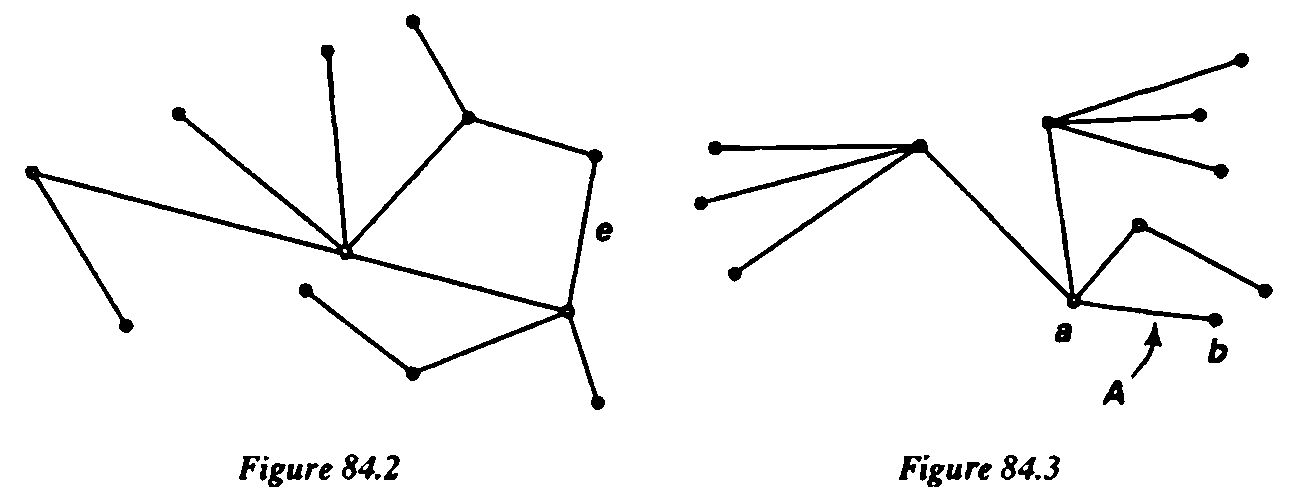
\includegraphics[width=0.45\linewidth]{images/84.2.png}\label{fig:84.2} &
   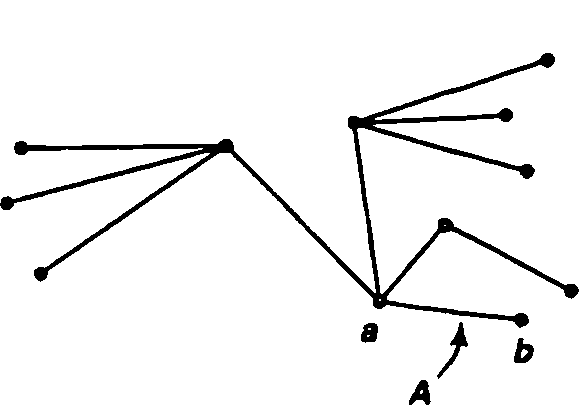
\includegraphics[width=0.45\linewidth]{images/84.3.png}\label{fig:84.3} \\[1em]
   \textbf{\textsl{Figure 84.2}} &
   \textbf{\textsl{Figure 84.3}}
  \end{tabular}
 \end{center}

\begin{lemma}
\label{lem:\thetheorem}
	If \(T\) is a tree in \(X\), and if \(A\) is an edge of \(X\) that intersects \(T\) in a single vertex, then \(T \cup A\) is a tree in \(X\). Conversely, if \(T\) is a finite tree in \(X\) that consists of more than one edge, then there is a tree \(T_{0}\) in \(X\) and an edge \(A\) of \(X\) that intersects \(T_{0}\) in a single vertex, such that \(T = T_{0} \cup A\).
\end{lemma}

\begin{proof}
	Suppose \(T\) is a tree in \(X\) and \(A\) is an edge that intersects \(T\) in a single vertex. Clearly \(T \cup A\) is connected; we show it contains no closed reduced edge paths. Let \(a\) and \(b\) be the end points of \(A\), with \(\{ a\} = T \cap A\). See \hyperref[fig:84.3]{Figure 84.3}. Suppose \(x_{0},\ldots ,x_{n} =\) \(x_{0}\) is the vertex sequence of a closed reduced edge path in \(T \cup A\). If none of the vertices \(x_{i}\) equals \(b\), then the edge path lies in \(T\), contrary to hypothesis. If \(x_{i} = b\) for some \(i\) with \(0 < i < n\), then we must have \(x_{i - 1} = a\) and \(x_{i + 1} = a\) ; hence the edge path is not reduced, contrary to hypothesis. Finally, if \(x_{0} = b = x_{n}\) and \(x_{i} \neq b\) for \(i = 1,\ldots, n - 1\), then \(x_{1} = a\) and \(x_{n - 1} = a\), and the vertex sequence \(x_{1},\ldots ,x_{n - 1}\) specifies a closed reduced edge path in \(T\), again contrary to hypothesis.
Now let \(T\) be a finite tree in \(X\) having more than one edge. First, we show that some vertex \(b\) of \(T\) belongs to only one edge of \(T\). If this is not the case, we can construct an edge path in \(T\) as follows: Begin with a vertex \(x_{0}\) of \(T\) ; then choose an edge \(e_{1}\) of \(T\) having \(x_{0}\) as an end point. Orient \(e_{1}\) so \(x_{0}\) is its initial vertex. Let \(x_{1}\) be the other end point of \(e_{1}\), and let \(e_{2}\) be an edge of \(T\) different from \(e_{1}\) having \(x_{1}\) as a vertex. Orient \(e_{2}\) so \(x_{1}\) is its initial vertex. Similarly continue. No two successive terms of the sequence \(e_{1},e_{2},\ldots\) are opposite orientations of the same edge of \(T\). Since \(T\) is finite, there must be an index \(n\) such that \(x_{n} = x_{i}\) for some \(i < n\). Then the sequence of vertices \(x_{i},x_{i + 1},\ldots ,x_{n}\) determines a closed reduced edge path in \(T\), contrary to hypothesis. See \hyperref[fig:84.4]{Figure 84.4}.

Let \(b\) be a vertex of \(T\) belonging to only one edge \(A\) of \(T\), and let \(T_{0}\) consist of all edges of \(T\) different from \(A\). Then \(T = T_{0} \cup A\). Because \(T\) is connected, \(T_{0}\) must intersect \(A\) in its other vertex \(a\). We show \(T_{0}\) is a tree. Clearly \(T_{0}\) contains no closed reduced edge paths, because \(T\) contains none. Furthermore, \(T_{0}\) is connected. For if \(T_{0}\) were the union of two disjoint closed sets \(C\) and \(D\), the point \(a\) would lie in one of them, say \(C\). Then \(C \cup A\) and \(D\) would be disjoint closed sets whose union is \(T\), contrary to the fact that \(T\) is connected.

\munkresfig[0.7]{84.4}[Figure 84.4]
\end{proof}
\begin{theorem}
\label{thm:\thetheorem}
	Any tree \(T\) is simply connected.
\end{theorem}

\begin{proof}
	We first consider the case where \(T\) is a finite tree. If \(T\) consists of a single edge, then \(T\) is simply connected. If \(T\) has \(n\) edges with \(n > 1\), there is an edge \(A\) of \(T\) such that \(T = T_{0} \cup A\), where \(T_{0}\) is a tree with \(n - 1\) edges and \(T_{0} \cap A\) is a single vertex. Then \(T_{0}\) is a deformation retract of \(T\). Since \(T_{0}\) is simply connected by the induction hypothesis, so is \(T\).
To prove the general case, let \(f\) be a loop in \(T\). The image set of \(f\) is compact and connected, so it is contained in a finite connected subgraph \(Y\) of \(T\). Now \(Y\) contains no closed reduced edge paths, because \(T\) contains none. Thus \(Y\) is a tree. Since \(Y\) is finite, it is simply connected. Hence \(f\) is path homotopic to a constant in \(Y\).
\end{proof}
\begin{definition}
	A tree \(T\) in \(X\) is maximal if there is no tree in \(X\) that properly contains \(T\).
\end{definition}

\begin{theorem}
\label{thm:\thetheorem}
	Let \(X\) be a connected graph. A tree \(T\) in \(X\) is maximal if and only if it contains all the vertices of \(X\).
\end{theorem}

\begin{proof}
	Suppose \(T\) is a tree in \(X\) that contains all the vertices of \(X\). If \(Y\) is a subgraph of \(X\) that properly contains \(T\), we show that \(Y\) contains a closed reduced edge path; it follows that \(T\) is maximal. Let \(A\) be an edge of \(Y\) that is not in \(T\) ; by hypothesis, the end points \(a\) and \(b\) of \(A\) belong to \(T\). Since \(T\) is connected, we can choose a reduced edge path \(e_{1},\ldots ,e_{n}\) in \(T\) from \(a\) to \(b\). If we follow this sequence by the edge \(A\), oriented from \(b\) to \(a\), we obtain a closed reduced edge path in \(Y\).
Now let \(T\) be a tree in \(X\) that does not contain all the vertices of \(X\). We show \(T\) is not maximal. Let \(x_{0}\) be a vertex of \(X\) not in \(T\). Since \(X\) is connected, we may choose an edge path in \(X\) from \(x_{0}\) to a vertex of \(T\), specified by the sequence of vertices \(x_{0}\), \(\ldots ,x_{n}\). Let \(i\) be the smallest index such that \(x_{i} \in T\). Let \(A\) be the edge of \(X\) with vertices \(x_{i - 1}\) and \(x_{i}\). Then \(T \cup A\) is a tree in \(X\), by the preceding lemma, and \(T \cup A\) properly contains \(T\).
\end{proof}
\begin{theorem}
\label{thm:\thetheorem}
	If \(X\) is a linear graph, every tree \(T_{0}\) in \(X\) is contained in a maximal tree in \(X\).
\end{theorem}

\begin{proof}
	We apply Zorn's lemma to the collection \(\mathcal{T}\) of all trees in \(X\) that contain \(T_{0}\), strictly partially ordered by proper inclusion. To show this collection has a maximal element, we need only prove the following:
If \(\mathcal{T}^{\prime }\) is a subcollection of \(\mathcal{T}\) that is simply ordered by proper inclusion, then the union \(Y\) of the elements of \(\mathcal{T}^{\prime }\) is a tree in \(X\).

To begin, we note that since \(Y\) is a union of subgraphs of \(X\), it is a subgraph of \(X\). Second, since \(Y\) is a union of connected spaces that contain the connected space \(T_{0}\), the space \(Y\) is connected.

Finally, we suppose that \(e_{1},\ldots ,e_{n}\) is a closed reduced edge path in \(Y\) and derive a contradiction. For each \(i\), choose an element \(T_{i}\) of \(\mathcal{T}^{\prime }\) that contains \(e_{i}\). Because \(\mathcal{T}^{\prime }\) is simply ordered by proper inclusion, one of the trees \(T_{1},\ldots ,T_{n}\), say \(T_{j}\), contains all the others. But then \(e_{1},\ldots ,e_{n}\) is a closed reduced edge path in \(T_{j}\), contrary to hypothesis.

Now we compute the fundamental group of a graph. We need the following result.
\end{proof}
\begin{lemma}
\label{lem:\thetheorem}
	Suppose \(X = U \cup V\), where \(U\) and \(V\) are open sets of \(X\). Suppose that \(U \cap V\) is the union of two disjoint open path-connected sets \(A\) and \(B\), that \(\alpha\) is a path in \(U\) from the point \(a\) of \(A\) to the point \(b\) of \(B\), and that \(\beta\) is a path in \(V\) from \(b\) to \(a\). If \(U\) and \(V\) are simply connected, then the class \([ {\alpha * \beta }]\) generates \({\pi }_{1}( {X,a})\).
\end{lemma}

\begin{proof}
	The situation is similar to that of \hyperref[thm:59.1]{Theorem 59.1}, except that \(U \cap V\) has two path components instead of one. The proof is also similar.
Let \(f\) be a loop in \(X\) based at \(a\). Choose a subdivision \(0 = a_{0} < a_{1} < \cdots < a_{n} =\) 1 of \([ {0,1}]\) such that for each \(i,f( a_{i}) \in U \cap V\) and \(f\) maps \([ {a_{i - 1},a_{i}}]\) into either \(U\) or \(V\). Let \(f_{i}\) be the positive linear map of \([ {0,1}]\) onto \([ {a_{i - 1},a_{i}}]\) followed by \(f\) ; then \([ f] = [ f_{1}] * \cdots * [ f_{n}]\). For \(i = 1,\ldots, n - 1\), choose a path \({\alpha }_{i}\) in either \(A\) or \(B\) from \(a\) or \(b\) to \(f( a_{i})\) ; choose \({\alpha }_{0}\) and \({\alpha }_{n}\) to be the constant paths at \(a\). Then set

\[
g_{i} = {\alpha }_{i - 1} * ( {f_{i} * \bar{\alpha }_{i}}).
\]

By direct computation, \([ f] = [ g_{1}] * \cdots * [ g_{n}]\). Because \(g_{i}\) is a path in \(U\) or in \(V\) with end points in the set \(\{ a,b\}\), and because \(U\) and \(V\) are simply connected, \(g_{i}\) is path homotopic either to a constant or to \(\alpha ,\beta ,\bar{\alpha }\), or \(\bar{\beta }\). It follows that either \([ f]\) is trivial, or it equals a positive power of \([ {\alpha * \beta }]\) or \([ {\bar{\beta } * \bar{\alpha }}]\). Hence \([ {\alpha * \beta }]\) generates the group \({\pi }_{1}( {X,a})\). See \hyperref[fig:84.5]{Figure 84.5}.

\munkresfig[1.0]{84.5}[Figure 84.5]
\end{proof}
\begin{theorem}
\label{thm:\thetheorem}
	Let \(X\) be a connected graph that is not a tree. Then the fundamental group of \(X\) is a nontrivial free group. Indeed, if \(T\) is a maximal tree in \(X\), then the fundamental group of \(X\) has a system of free generators that is in bijective correspondence with the collection of edges of \(X\) that are not in \(T\).
\end{theorem}

\begin{proof}
	Let \(T\) be a maximal tree in \(X\) ; it contains all the vertices of \(X\). Let \(x_{0}\) be a fixed vertex of \(T\). For each vertex \(x\) of \(X\), choose a path \({\gamma }_{x}\) in \(T\) from \(x_{0}\) to \(x\). Then for each edge \(A\) of \(X\) that is not in \(T\), define a loop \(g_{A}\) in \(X\) as follows. Orient \(A\) ; let \(f_{A}\) be the linear path in \(A\) from its initial end point \(x\) to its final end point \(y\) ; and set
\[
g_{A} = {\gamma }_{x} * ( {f_{A} * \bar{\gamma }_{y}}).
\]

We show that the classes \([ g_{A}]\) form a system of free generators for \({\pi }_{1}( {X,x_{0}})\).

Step 1. We first prove the theorem when the edges of \(X\) not in \(T\) are finite in number. We proceed by induction. The induction step is easy, so we consider it first.

Let \(A_{1},\ldots ,A_{n}\) be the edges of \(X\) not in \(T\), where \(n > 1\). Orient these edges and let \(g_{i}\) denote the loop \(g_{A_{i}}\). For each \(i\), choose a point \(p_{i}\) interior to \(A_{i}\). Let

\[
U = X - p_{2} - \cdots - p_{n}\;\text{ and }\;V = X - p_{1}.
\]

Then \(U\) and \(V\) are open in \(X\), and the space \(U \cap V = X - p_{1} - \cdots - p_{n}\) is simply connected, since it has \(T\) as a deformation retract. Therefore, \({\pi }_{1}( {X,x_{0}})\) is the free product of the groups \({\pi }_{1}( {U,x_{0}})\) and \({\pi }_{1}( {V,x_{0}})\), by \hyperref[cor:70.3]{Corollary 70.3}.

The space \(U\) has \(T \cup {A}_{1}\) as a deformation retract, so \({\pi }_{1}( {U,x_{0}})\) is free on the generator \([ g_{1}]\), as we shall prove in Step 2. The space \(V\) has \(T \cup {A}_{2} \cup \cdots \cup {A}_{n}\) as a deformation retract, so it is free on the generators \([ g_{2}] ,\ldots ,[ g_{n}]\), by the induction hypothesis. It follows from \hyperref[thm:69.2]{Theorem 69.2} that \({\pi }_{1}( {X,x_{0}})\) is free on the generators \([ g_{1}]\), \(\ldots ,[ g_{n}]\). See \hyperref[fig:84.6]{Figure 84.6}.

\munkresfig[0.7]{84.6}[Figure 84.6]
Step 2. We now consider the case where there is only one edge \(D\) of \(X\) that is not in \(T\). This step is more difficult. Orient \(D\). We show \({\pi }_{1}( {X,x_{0}})\) is infinite cyclic with generator \([ g_{D}]\).

Let \(a_{0}\) and \(a_{1}\) be the initial and final points of \(D\), respectively. Let us write \(D\) as the union of three arcs: \(D_{1}\), with end points \(a_{0}\) and \(a\), \(D_{2}\), with end points \(a\) and \(b\), and \(D_{3}\), with end points \(b\) and \(a_{1}\). See \hyperref[fig:84.7]{Figure 84.7}. Let \(f_{1},f_{2}\), and \(f_{3}\) be the linear paths in \(D\) from \(a_{0}\) to \(a\), and \(a\) to \(b\), and \(b\) to \(a_{1}\), respectively. We apply the preceding theorem to compute \({\pi }_{1}( {X,a})\).

\munkresfig[0.8]{84.7}[Figure 84.7]
Choose a point \(p\) interior to the arc \(D_{2}\). Set \(U = D - a_{0} - a_{1}\) and \(V = X - p\). Then \(U\) and \(V\) are open sets in \(X\) whose union is \(X\). The space \(U\) is simply connected because it is an open arc. And the space \(V\) is simply connected because it has the tree \(T\) as a deformation retract. The space \(U \cap V\) equals \(U - p\) ; it has two path components; let \(A\) be the one containing \(a\) and let \(B\) be the one containing \(b\). Then the hypotheses of the preceding lemma are satisfied. The path \(\alpha = f_{2}\) is a path in \(U\) from \(a\) to \(b\). If we set \({\gamma }_{0} = {\gamma }_{a_{0}}\) and \({\gamma }_{1} = {\gamma }_{a_{1}}\), then the path \(\beta = ( {f_{3} * ( {\bar{\gamma }_{1} * ( {{\gamma }_{0} * f_{1}}) }) })\) is a path in \(V\) from \(b\) to \(a\). Therefore, \({\pi }_{1}( {X,a})\) is generated by the class

\[
[ {\alpha * \beta }] = [ f_{2}] * [ f_{3}] * [ \bar{\gamma }_{1}] * [ {\gamma }_{0}] * [ f_{1}] .
\]

It follows that \({\pi }_{1}( {X,x_{0}})\) is generated by \(\widehat{\delta }[ {\alpha * \beta }]\), where \(\delta\) is the path \(\bar{f}_{1} * \bar{\gamma }_{0}\) from \(a\) to \(x_{0}\). We compute this path-homotopy class as follows:

\[
\widehat{\delta }[ {\alpha * \beta }] = [ {{\gamma }_{0} * f_{1}}] * [ {\alpha * \beta }] * [ {\bar{f}_{1} * \bar{\gamma }_{0}}]
\]

\[
= [ {\gamma }_{0}] * [ {f_{1} * ( {f_{2} * f_{3}}) }] * [ \bar{\gamma }_{1}]
\]

\[
= [ {\gamma }_{0}] * [ f_{D}] * [ \bar{\gamma }_{1}]
\]

\[
= [ g_{D}] \text{.}
\]

Therefore, \([ g_{D}]\) generates \({\pi }_{1}( {X,x_{0}})\).

It remains to show that the element \([ g_{D}]\) has infinite order, so that \({\pi }_{1}( {X,x_{0}})\) is infinite cyclic. One can apply \hyperref[thm:63.1]{Theorem 63.1} (which we used in proving the Jordan curve theorem), which states that \([ {\alpha * \beta }]\) has infinite order in \({\pi }_{1}( {X,a})\). Alternatively (and more easily), one can consider the map \(\pi : X \rightarrow {S}^{1}\) that collapses the tree \(T\) to a single point \(p\) and maps the open arc Int \(D\) homeomorphically onto \(S^{1} - p\). Then \(\pi \circ {\gamma }_{0}\) and \(\pi \circ {\bar{\gamma }}_{1}\) are constant paths, so that

\[
{\pi }_{ * }( [ g_{D}] ) = [ {\pi \circ {f}_{D}}] .
\]

This class generates \({\pi }_{1}( {S^{1},p})\). It follows that \([ g_{D}]\) has infinite order in \({\pi }_{1}( {X,x_{0}})\).

Step 3. Now we consider the situation where the collection of edges of \(X\) not in \(T\) is infinite. The proof in this case is so similar to the corresponding proof for an infinite wedge of circles that we omit the details. (See \hyperref[thm:71.3]{Theorem 71.3}.) The crucial facts are these: Any loop in \(X\) based at \(x_{0}\) lies in the space

\[
X( {{\alpha }_{1},\ldots ,{\alpha }_{n}}) = T \cup {A}_{{\alpha }_{1}} \cup \cdots \cup {A}_{{\alpha }_{n}}
\]

for some finite set of indices \({\alpha }_{i}\), and any path homotopy between such loops also lies in such a space. By this means the general case is reduced to the finite case.
\end{proof}
\section*{Exercises}
\begin{enumerate}[itemsep=0.4em, parsep=0pt, topsep=0pt, partopsep=0pt, leftmargin=*, label=\arabic*., ref=\arabic*]
\item Give an example to show that the second part of \hyperref[lem:84.2]{Lemma 84.2} need not hold if \(T\) is infinite.
\item What is the cardinality of a system of free generators for the fundamental group of the complete graph on \(n\) vertices? of the utilities graph? (See \S\ 64.)
\item Let \(X\) be the wedge of two circles; let \(p : E \rightarrow X\) be a covering map. The fundamental group of \(E\) maps isomorphically under \(p_{ * }\) onto a subgroup \(H\) of the fundamental group of \(X\) ; the latter is free on two generators \(\alpha\) and \(\beta\).
 \begin{enumerate}[itemsep=0.2em, parsep=0pt, topsep=0pt, partopsep=0pt, leftmargin=*, label=(\alph*), align=left]
 \item For each of the four covering spaces \(E\) given in Exercise 2 of \S\ 81, determine the cardinality of a system of free generators for the fundamental group of \(E\).
 \item For each of these covering spaces, find, in terms of \(\alpha\) and \(\beta\), a system of free generators for the subgroup \(H\) of the fundamental group of \(X\).
 \end{enumerate}
\end{enumerate}
\booksection{85}{Subgroups of Free Groups}

We now prove our main theorem, to the effect that a subgroup \(H\) of a free group \(F\) is free. The method of proof, remarkably enough, will give us some information about the cardinality of a system of free generators for \(H\), when the cardinality of a system of free generators for \(F\) is known.

\begin{theorem}
\label{thm:\thetheorem}
	If \(H\) is a subgroup of a free group \(F\), then \(H\) is free.
\end{theorem}

\begin{proof}
	Let \(\{ \alpha \mid \alpha \in J\}\) be a system of free generators for \(F\). Let \(X\) be a wedge of circles \(S_{\alpha }\), one for each \(\alpha \in J\) ; let \(x_{0}\) be their common point. We can give \(X\) the structure of a linear graph by breaking each circle \(S_{\alpha }\) into three arcs, two of which have \(x_{0}\) as an end point. The function that assigns to each \(\alpha\), a loop generating \({\pi }_{1}( {S_{\alpha },x_{0}})\), induces an isomorphism of \(F\) with \({\pi }_{1}( {X,x_{0}})\). Therefore we may as well assume that \(F\) equals the group \({\pi }_{1}( {X,x_{0}})\).
The space \(X\) is path connected, locally path connected, and semilocally simply connected. Therefore \hyperref[thm:82.1]{Theorem 82.1} applies to show that there exists a path-connected covering space \(p : E \rightarrow X\) of \(X\) such that, for some point \(e_{0}\) of \(p^{-1}( x_{0})\),

\[
p_{ * }( {{\pi }_{1}( {E,e_{0}}) }) = H
\]

Since \(p_{ * }\) is a monomorphism, \({\pi }_{1}( {E,e_{0}})\) is isomorphic to \(H\).

The space \(E\) is a linear graph, by \hyperref[thm:83.4]{Theorem 83.4}. Then \hyperref[thm:84.7]{Theorem 84.7} implies that its fundamental group is a free group.
\end{proof}
\begin{definition}
	If \(X\) is a finite linear graph, we define the Euler number of \(X\) to be the number of vertices of \(X\) minus the number of edges. It is commonly denoted by the Greek letter chi, as \(\chi ( X)\).
\end{definition}

\begin{lemma}
\label{lem:\thetheorem}
	If \(X\) is a finite, connected linear graph, then the cardinality of a system of free generators for the fundamental group of \(X\) is \(1 - \chi ( X)\).
\end{lemma}

\begin{proof}
	Step 1. We first show that for any finite tree \(T\), we have \(\chi ( T) = 1\). We proceed by induction on the number \(n\) of edges in \(T\). If \(n = 1\), then \(T\) has one edge and two vertices, so \(\chi ( T) = 1\). If \(n > 1\), we can write \(T = T_{0} \cup A\), where \(T_{0}\) is a tree having \(n - 1\) edges, and \(A\) is an edge that intersects \(T_{0}\) in a single vertex. We have \(\chi ( T_{0}) = 1\) by the induction hypothesis. The graph \(T\) has one more edge and one more vertex than \(T_{0}\) ; hence \(\chi ( T) = \chi ( T_{0})\).
Step 2. We prove the theorem. Given \(X\), let \(T\) be a maximal tree in \(X\). If \(X = T\), we are finished. Otherwise, let \(A_{1},\ldots ,A_{n}\) be the edges of \(X\) that are not in \(T\). Then the fundamental group of \(X\) has a system of \(n\) free generators. On the other hand, \(X\) and \(T\) have exactly the same vertex set, and \(X\) has \(n\) more edges than \(T\). Hence,

\[
\chi ( X) = \chi ( T) - n = 1 - n
\]

so that \(n = 1 - \chi ( X)\).
\end{proof}
\begin{definition}
	Let \(H\) be a subgroup of the group \(G\). If the collection \(G/H\) of right cosets of \(H\) in \(G\) is finite, its cardinality is called the index of \(H\) in \(G\). (The collection of left cosets of \(H\) in \(G\) has the same cardinality, of course.)
\end{definition}

\begin{theorem}
\label{thm:\thetheorem}
	Let \(F\) be a free group with \(n + 1\) free generators; let \(H\) be a subgroup of \(F\). If \(H\) has index \(k\) in \(F\), then \(H\) has \({kn} + 1\) free generators.
\end{theorem}

\begin{proof}
	We apply the construction given in the proof of \hyperref[thm:85.1]{Theorem 85.1}. We can assume that \(F = {\pi }_{1}( {X,x_{0}})\), where \(X\) is a linear graph whose underlying space is a wedge of \(n + 1\) circles. Given \(H\), we choose a path-connected covering space \(p : E \rightarrow X\) such that \(p_{ * }( {{\pi }_{1}( {E,e_{0}}) }) = H\). Now the lifting correspondence
\[
\Phi : {\pi }_{1}( {X,x_{0}}) /H \rightarrow {p}^{-1}( x_{0})
\]

is a bijection. Therefore, \(E\) is a \(k\) -fold covering of \(X\).

The space \(E\) is also a linear graph. Given an edge \(A\) of \(X\), the path components of \(p^{-1}( A)\) are edges of \(E\), and each is mapped by \(p\) homeomorphically onto \(A\). Thus \(E\) has \(k\) times as many edges as \(X\), and \(k\) times as many vertices. It follows that \(\chi ( E) = {k\chi }( X)\). Since the fundamental group of \(X\) has \(n + 1\) free generators, the preceding lemma tells us that \(\chi ( X) = - n\). Then the number of free generators of the fundamental group of \(E\), which is isomorphic to \(H\), is

\[
1 - \chi ( E) = 1 - {k\chi }( X) = 1 + {kn}.
\]

Note that if \(F\) is a free group with a finite system of free generators and \(H\) is a subgroup of \(F\) such that \(F/H\) is infinite, then nothing can be said about the cardinality of a system of free generators for \(H\). It might be finite (for instance, if \(H\) is the trivial subgroup) or infinite (for instance, if \(H\) is the fundamental group of the covering space pictured in \exrefs{81}{2}).
\end{proof}
\section*{Exercises}
\begin{enumerate}[itemsep=0.4em, parsep=0pt, topsep=0pt, partopsep=0pt, leftmargin=*, label=\arabic*., ref=\arabic*]
\item Show that the Euler number of a finite linear graph \(X\) is a topological invariant of \(X\). [Hint: First consider the case where \(X\) is connected.]
\item Let \(F\) be a free group on two free generators \(\alpha\) and \(\beta\). Let \(H\) be the subgroup generated by \(\alpha\). Show that \(H\) has infinite index in \(F\).
\item Let \(p : \mathbb{R} \rightarrow {S}^{1}\) be the standard covering map; consider the covering map \(p \times p : \mathbb{R} \times \mathbb{R} \rightarrow {S}^{1} \times {S}^{1}\). Let \(b_{0} = ( {1,0}) \in {S}^{1}\) ; set \(X = ( {b_{0} \times {S}^{1}}) \cup ( {S^{1} \times {b}_{0}})\) ; let \(E = {( p \times p) }^{-1}( X)\) ; and let \(q : E \rightarrow X\) be the covering map obtained by restricting \(p \times p\). The fundamental group of \(X\) has free generators \(\alpha\) and \(\beta\), where \(\alpha\) is represented by a loop in \(b_{0} \times {S}^{1}\) and \(\beta\) by a loop in \(S^{1} \times {b}_{0}\). Find a system of free generators for the subgroup \(q_{ * }( {{\pi }_{1}( {E,e_{0}}) })\), where \(e_{0}\) is the origin in \(\mathbb{R}^{2}\).
\end{enumerate}